\def\green#1{{\bf #1}}
\def\magenta#1{{\it #1}}
\subsection {Kinds of machine assistance}
There are various forms of machine-assisted proof, and they need different approaches.
\begin{itemize}
\item \green{Experimental mathematics}: Humans design experiments for the computers
to carry out, in order to discover or test new conjectures.
\item \green{Human/machine collaborative proofs}: Humans reduce a proof to a large 
number of cases, or to a detailed computation, which the computer carries out.
\item \green{Formal proof verification}: Humans supply the steps of a proof
in a language such that the computer can verify that each step 
follows logically from previous steps.
\item \green{Formal proof discovery}: The computer searches for a chain
of deduction leading from provided axioms to a theorem.
\end{itemize}
\magenta{Cloud computing services} make it possible to do computations 
much larger than most people would be able to do with their 
own physical computers.

\begin{example}
My colleague Andrew Sutherland at MIT 
did a 300 core-year computation in 8 hours
using (a record) 580,000 cores of the Google Compute Engine 
for about \$20,000.
\rm 
As he says, 
\begin{quote}
``Having a computer that is 10 times as fast 
doesn't really change the way you do your research, but having a computer
that is 10,000 times as fast does.''
\end{quote}
\end{example}

\subsection {Large databases}
There are now many databases of mathematical facts, such as the Atlas of Finite Simple Groups \cite{Conwayetal1985} and the Online Encyclopedia of Integer Sequences \cite{Sloane2003,Sloane2007}. My personal tool is the LMFDB --- The L-functions and modular forms database (\url{www.lmfdb.org}).
\begin{figure}
	\caption{Modular Forms Database}
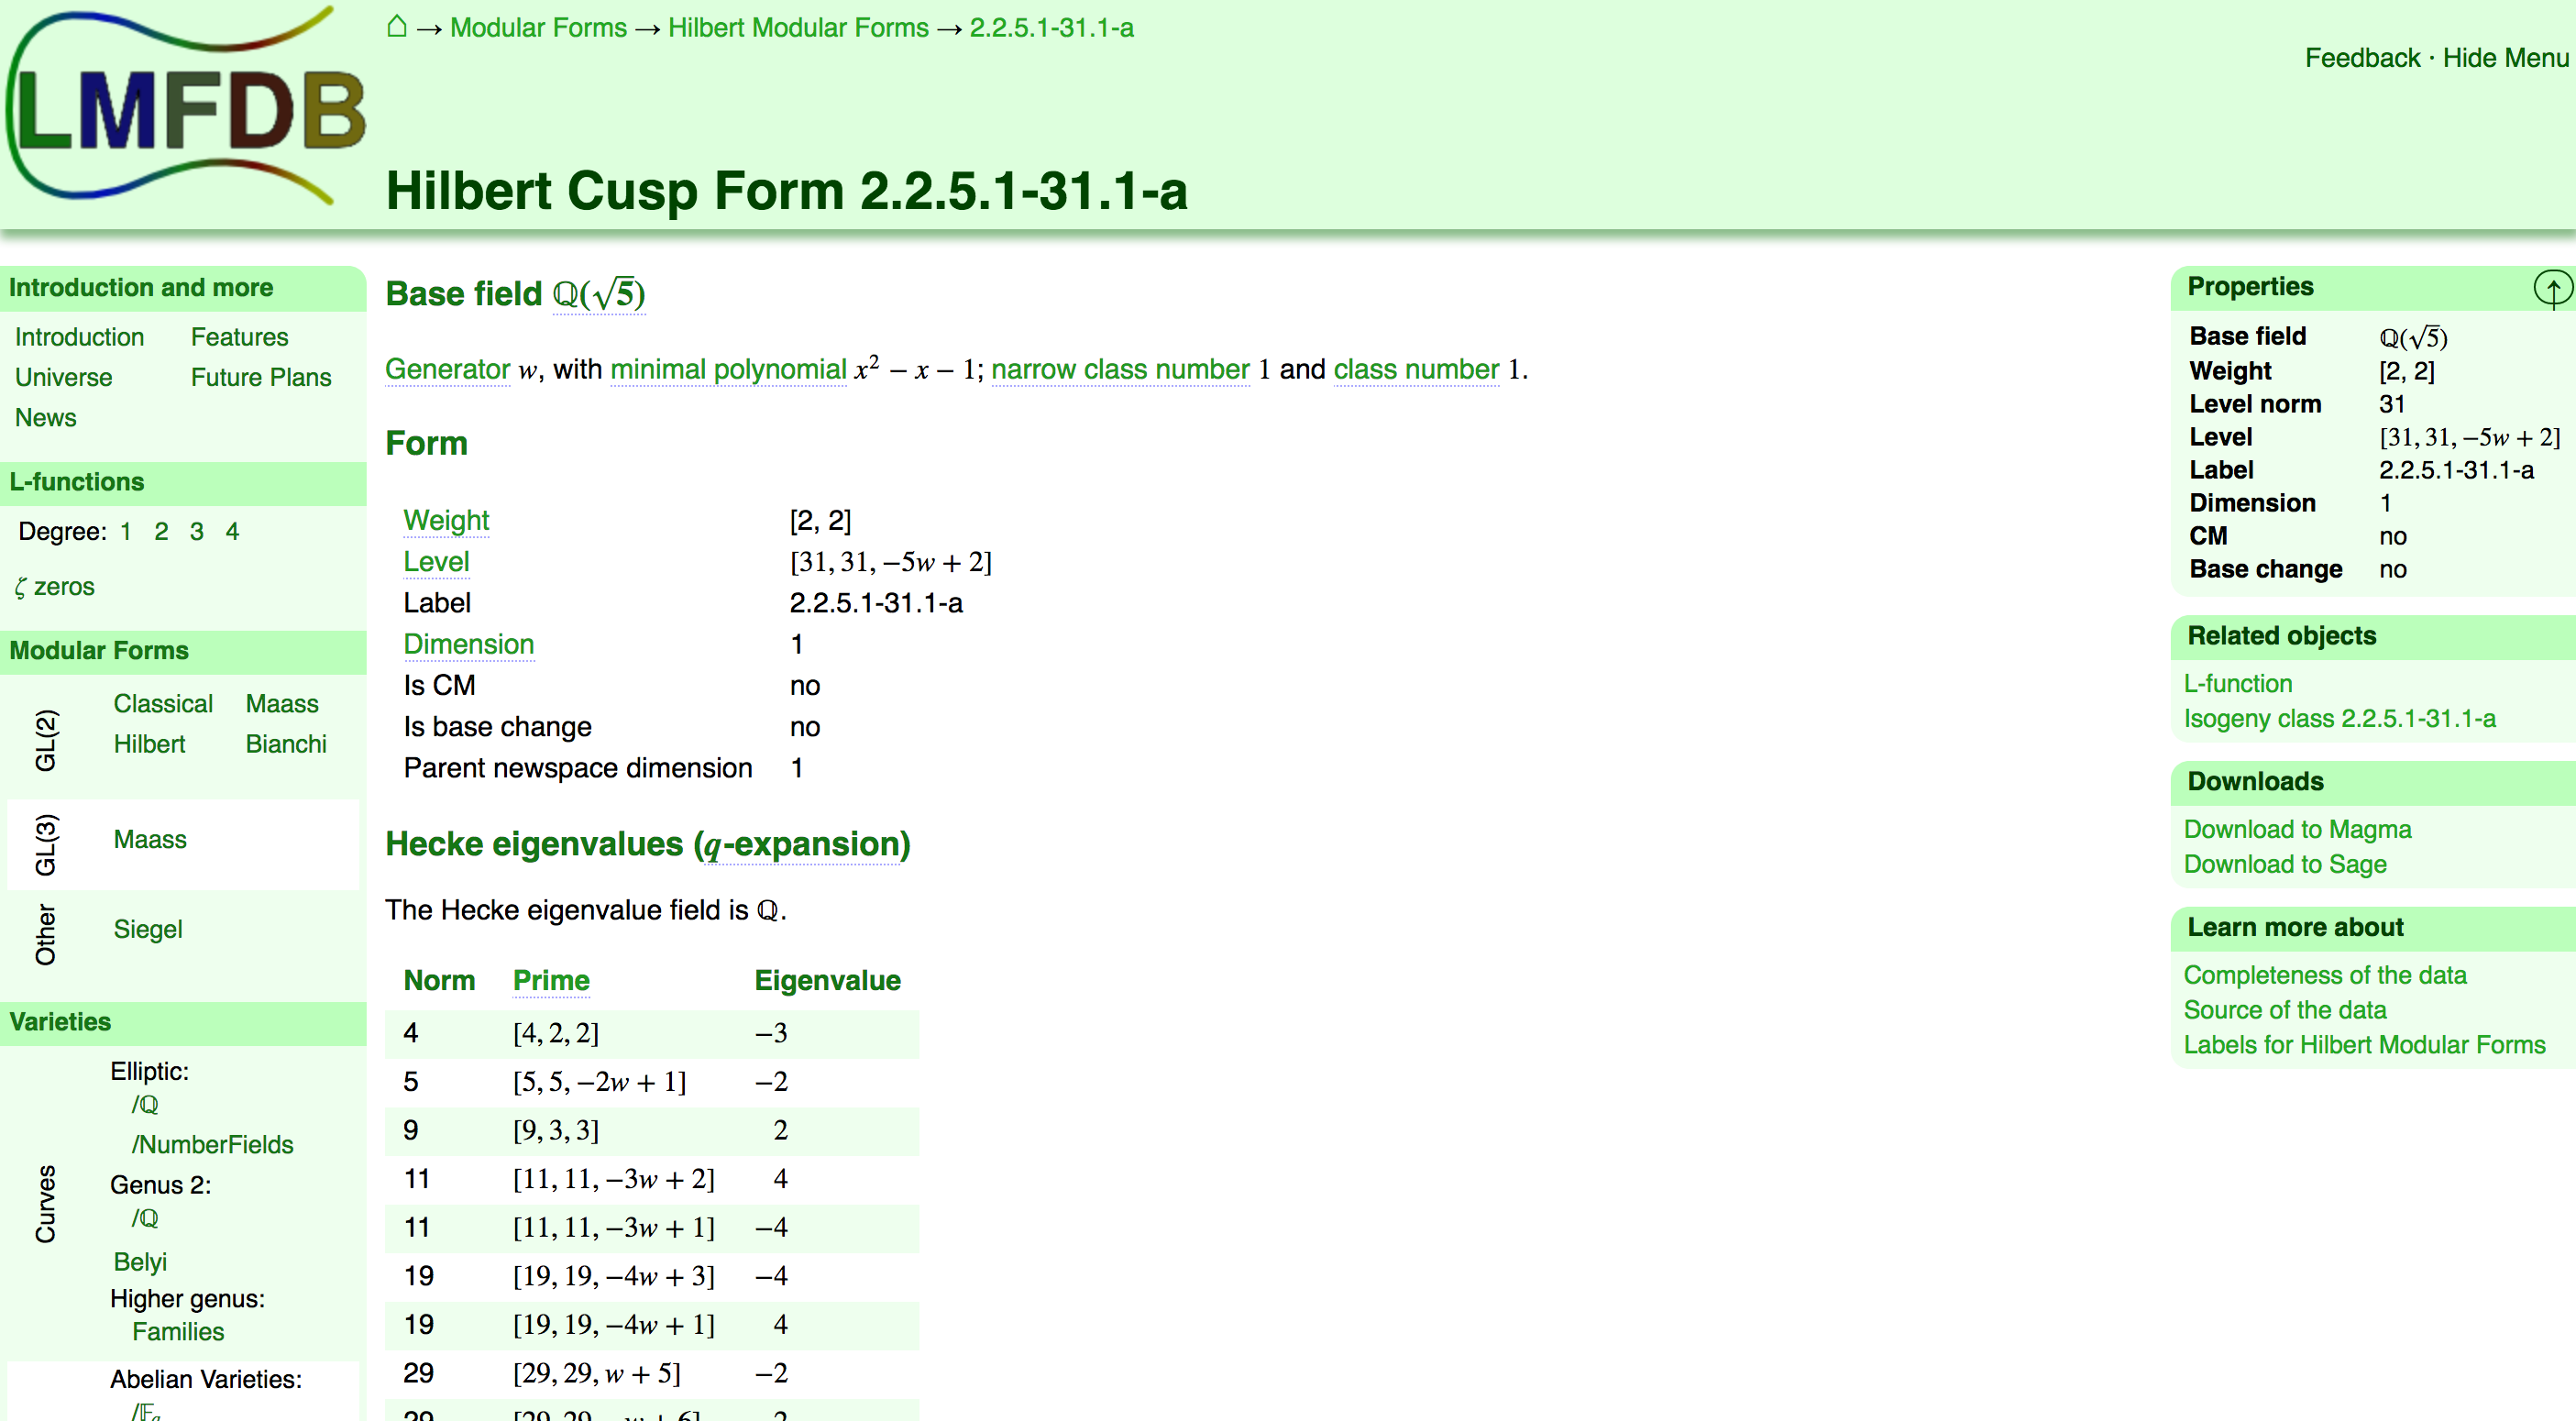
\includegraphics[scale=0.25]{LMFDB.png}
\end{figure}

\subsection {Refereeing computations}

Almost all math journals now publish papers depending on machine computations.
\begin{itemize}
\item
Should papers involving machine-assisted proofs 
be viewed as more or less suspect than purely human ones?
\item 
What if \magenta{the referee is not qualified} to check the computations,
e.g., by redoing them?
\item 
What if the computations are \magenta{too expensive} to do more than once?
\item 
What if the computation involves \magenta{proprietary software} (e.g., MAGMA)
for which there is no direct way to check that the algorithms
do what they claim to do?
\item 
Should one insist on \green{open-source software},
or even software that has gone through a \green{peer-review process}
(as in Sage, for instance)?
\item
In what form should computational proofs be published?
\end{itemize}

\subsection {Some opinions}

\begin{itemize}
\item
The burden should be on authors 
to provide understandable and verifiable code,
just as the burden is on authors to make their human-generated proofs 
understandable and verifiable.
\item 
Ideally, code should be written in a high-level computer algebra package
whose language is close to mathematics,
to minimize the computer proficiency demands on a potential reader.
\end{itemize}

{\bf Acknowledgements.} Many thanks are due to my colleague Andrew V. Sutherland.
